\documentclass[11pt]{exam}
\usepackage[utf8]{inputenc}
\usepackage{hyperref}
\usepackage{graphicx}
\usepackage[export]{adjustbox}

\title{Clustering en Weka}
\author{Laura Rodríguez Navas \\ rodrigueznavas@posgrado.uimp.es}
\date{\today}

\pagestyle{plain}

\begin{document}
	
\maketitle

En esta práctica se realiza un estudio acerca de la base de datos Iris. Esta BD se distribuye junto a la herramienta \href{https://www.cs.waikato.ac.nz/ml/weka/}{Weka}. 

\begin{questions}
	
% Pregunta 1
{\question Ejecuta el algoritmo SimpleKMeans usando la herramienta Weka con las distancias Euclídea y Manhattan.}

La BD está formada por 4 variables descriptivas y una variable clase. No se aplica preprocesamiento de datos ya que las variables descriptivas son numéricas y no existen valores perdidos en la BD. Además, como la variable de clase puede tomar tres valores, elegimos que el valor de \textit{k} sea igual a 3.

\renewcommand{\figurename}{Figura}

\begin{figure}[h]
	\centering
	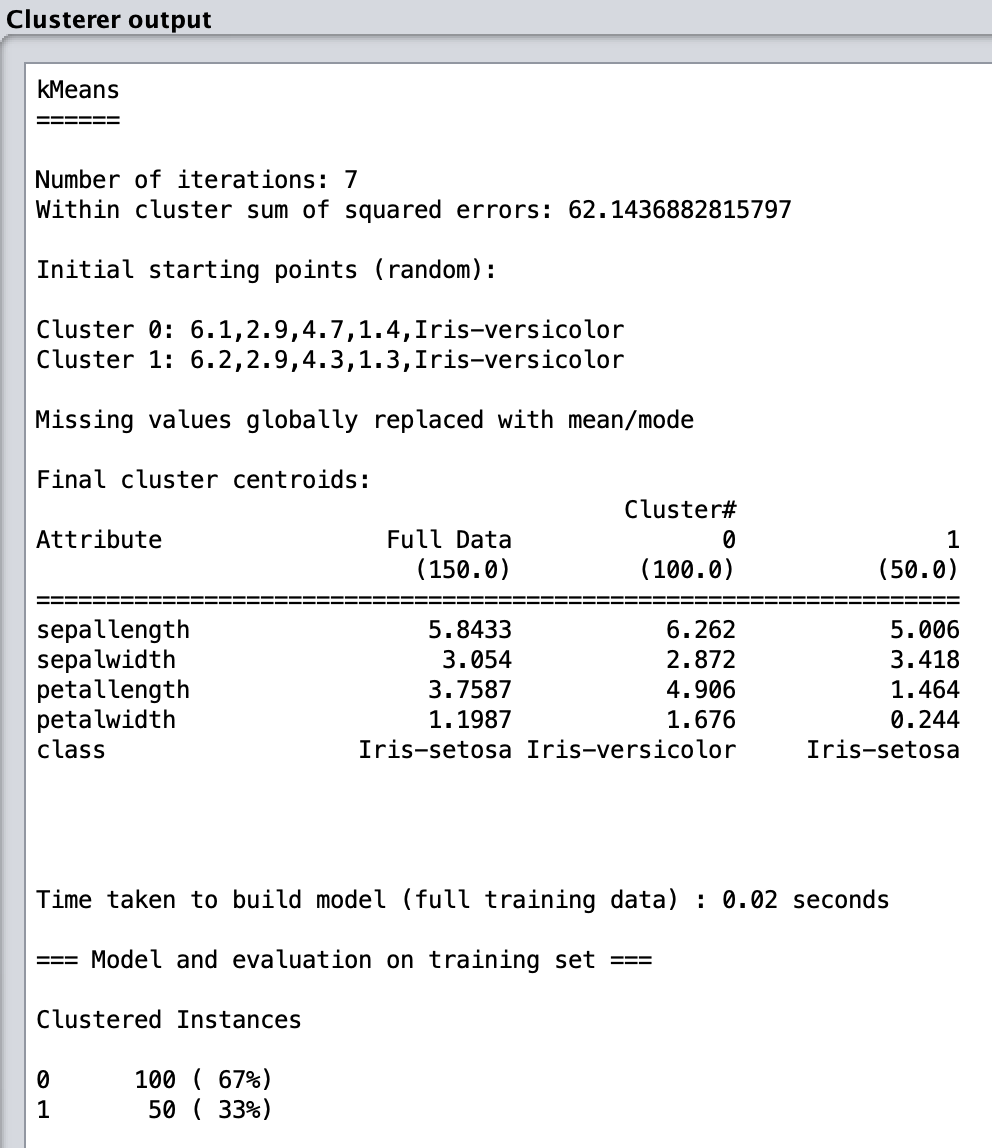
\includegraphics[width=0.6\textwidth]{kmeans_euclidea.png}
	\caption{KMeans con distancia Euclídea.}
	\label{Captura_1}
\end{figure}


\begin{figure}[h]
	\centering
	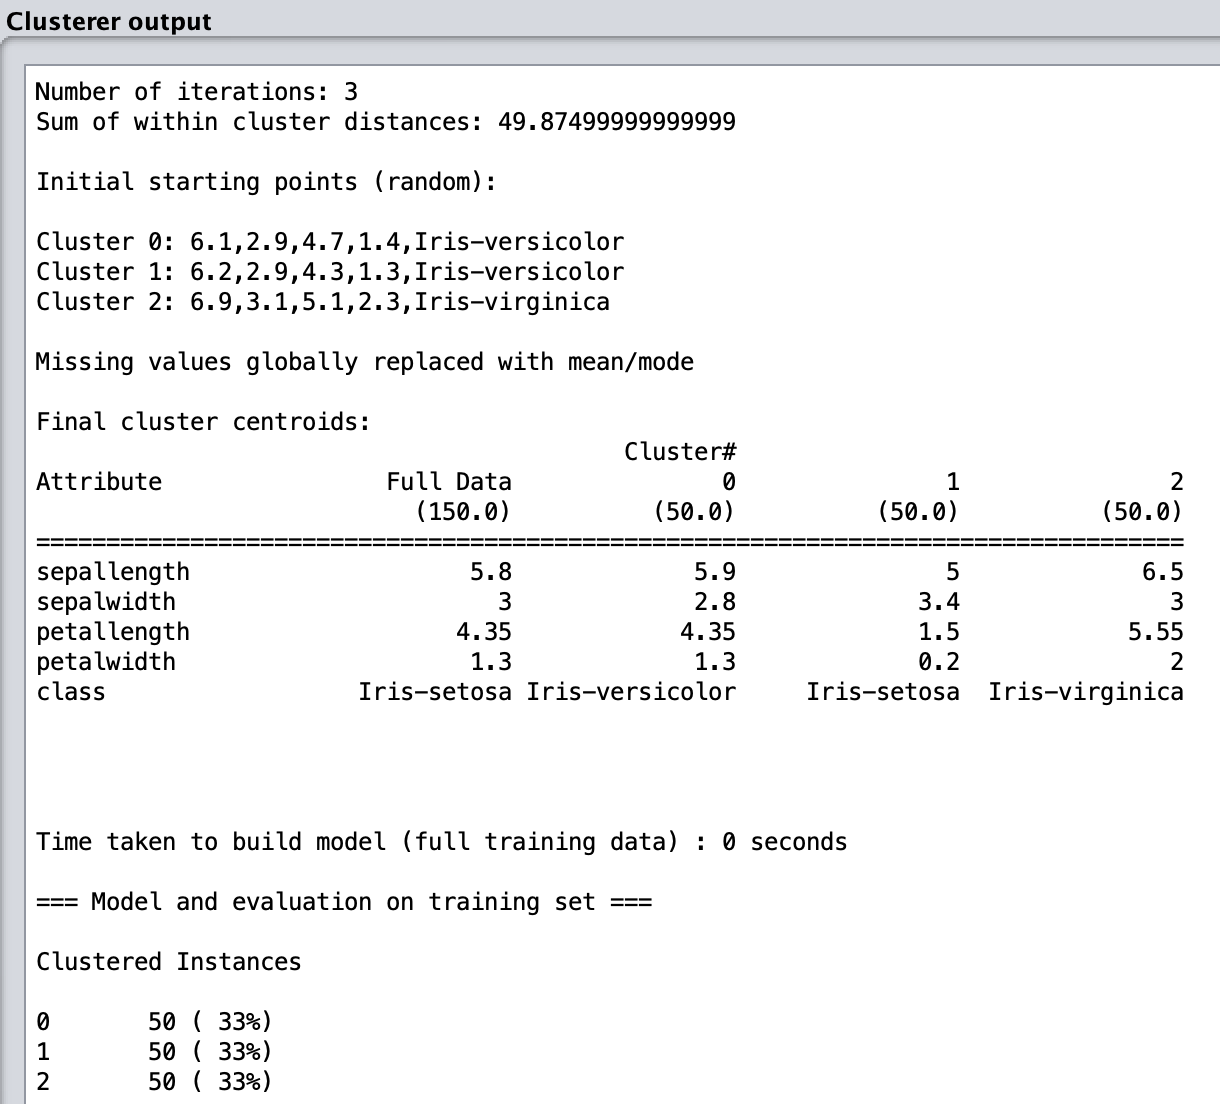
\includegraphics[width=0.6\textwidth]{kmeans_manhattan.png}
	\caption{KMeans con distancia Manhattan.}
	\label{Captura_2}
\end{figure}

\begin{parts}

\part ¿Cuántas instancias contiene cada grupo?

En la ejecución del algoritmo KMeans con distancia Euclídea (ver Figura \ref{Captura_1}) se han formado tres grupos: 0, 1 y 2. Los 3 grupos contienen 50 instancias cada uno. En la ejecución del algoritmo KMeans con distancia Manhattan (ver Figura \ref{Captura_2}) también se han formado los grupos 0, 1 y 2, con el mismo número de instancias cada uno.

\newpage
\part ¿Cuáles son los centroides?

Si nos volvemos a fijar en la figura \ref{Captura_1}, podemos observar los centroides de la ejecución de Kmeans con distancia Euclídea, y en la figura \ref{Captura_2}, podemos observar los centroides de la ejecución de Kmeans con distancia Manhattan. Se muestran más detalladamente en las siguientes figuras:

\begin{figure}[h]
	\centering
	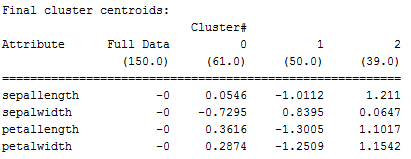
\includegraphics[width=0.45\textwidth]{kmeans_euclidea_centroides.png}
	\caption{KMeans centroides con distancia Euclídea.}
	\label{Captura_3}
	\bigbreak
	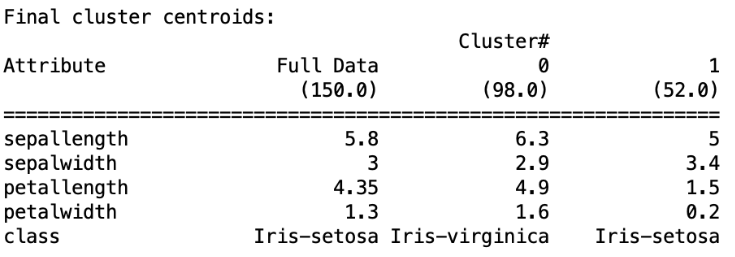
\includegraphics[width=0.45\textwidth]{kmeans_manhattan_centroides.png}
	\caption{KMeans centroides con distancia Manhattan.}
	\label{Captura_4}
\end{figure}

\newpage
\part Analiza los centroides. ¿Hay algo destacable en esos centroides? ¿Están los centroides separados en el espacio? ¿Tienen componentes similares?

Los centroides resultantes de la ejecución del algoritmo KMeans con distancia Euclídea y los centroides resultantes de la ejecución del algoritmo KMeans con distancia Manhattan son muy parecidos. Tienen componentes muy similares. Este comportamiento nos podría indicar que en la BD no existen \textit{outliers}, la distancia Manhattan se ve menos afectada por ellos (es más robusta), y al no presentar diferencias significantes con la distancia Euclídea, podría ser el motivo de tanta similitud.

En la figura \ref{Captura_5} se puede observar que los centroides están separados en el espacio. Aunque los centroides de los grupos 0 y 1 están más cercanos entre ellos. El centroide del grupo 2 es el que está más alejado.

\begin{figure}[h]
	\centering
	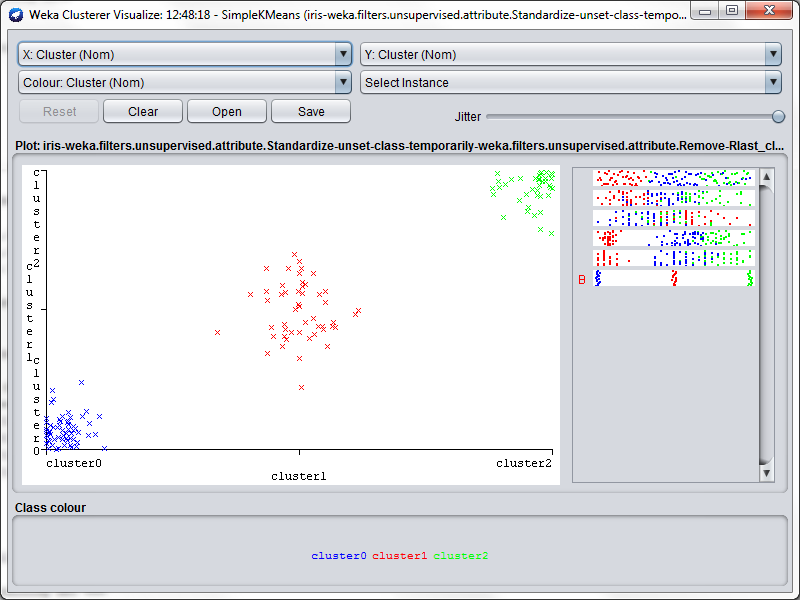
\includegraphics[width=0.6\textwidth]{kmeans_euclidea_centroides_graph.png}
	\caption{Representación de los centroides de KMeans con distancia Euclídea.}
	\label{Captura_5}
\end{figure}

\end{parts}

Nota: Solo se muestra la gráfica de los centroides resultantes de la ejecución del algoritmo KMeans con distancia Euclídea, porqué casi es igual a la gráfica de los centroides resultantes de la ejecución del algoritmo KMeans con distancia Manhattan.

% Pregunta 2
{\question Ejecuta el algoritmo HierarchicalClusterer con tipo de enlace completo y métrica de distancia euclídea, y visualice las gráficas de los puntos agrupados. ¿Alguno de ellas produce grupos bien diferenciados y con fronteras claras?}

Nota: Compara que el eje X instance\_number y el eje Y vaya variando y muestra cada una de las variables (debes adjuntar las imágenes).

Como se ha comentado anteriormente, la variable de clase puede tomar tres valores, así que volvemos a elegir \textit{k} igual a 3 para la ejecución del algoritmo (ver Figura \ref{Captura_6}).

\begin{figure}[h]
	\centering
	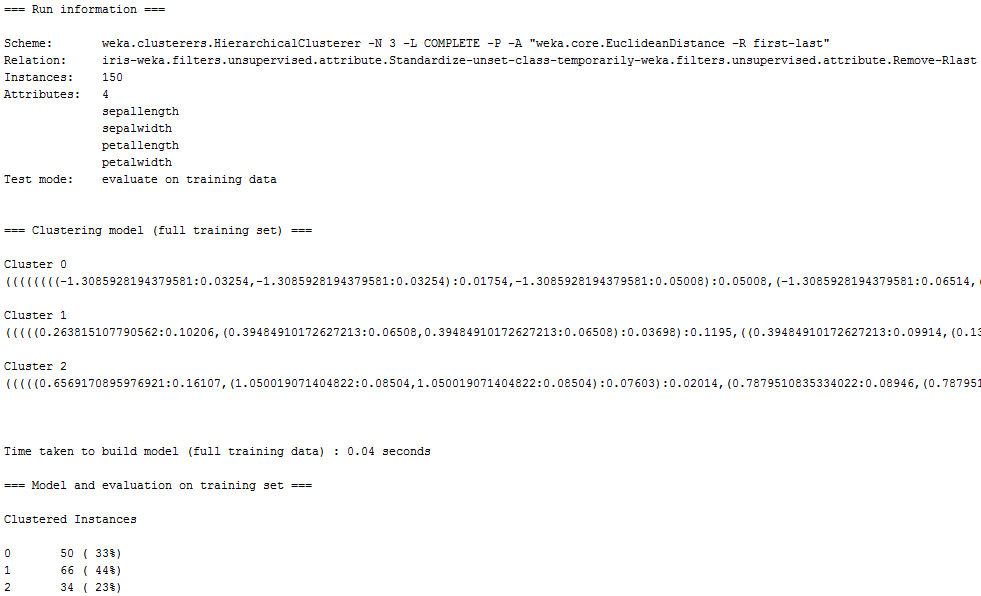
\includegraphics[width=0.6\textwidth]{hc_euclidea.png}
	\caption{Hierarchical Clustering con distancia Euclídea.}
	\label{Captura_6}
\end{figure}

\begin{figure}[h]
	\centering
	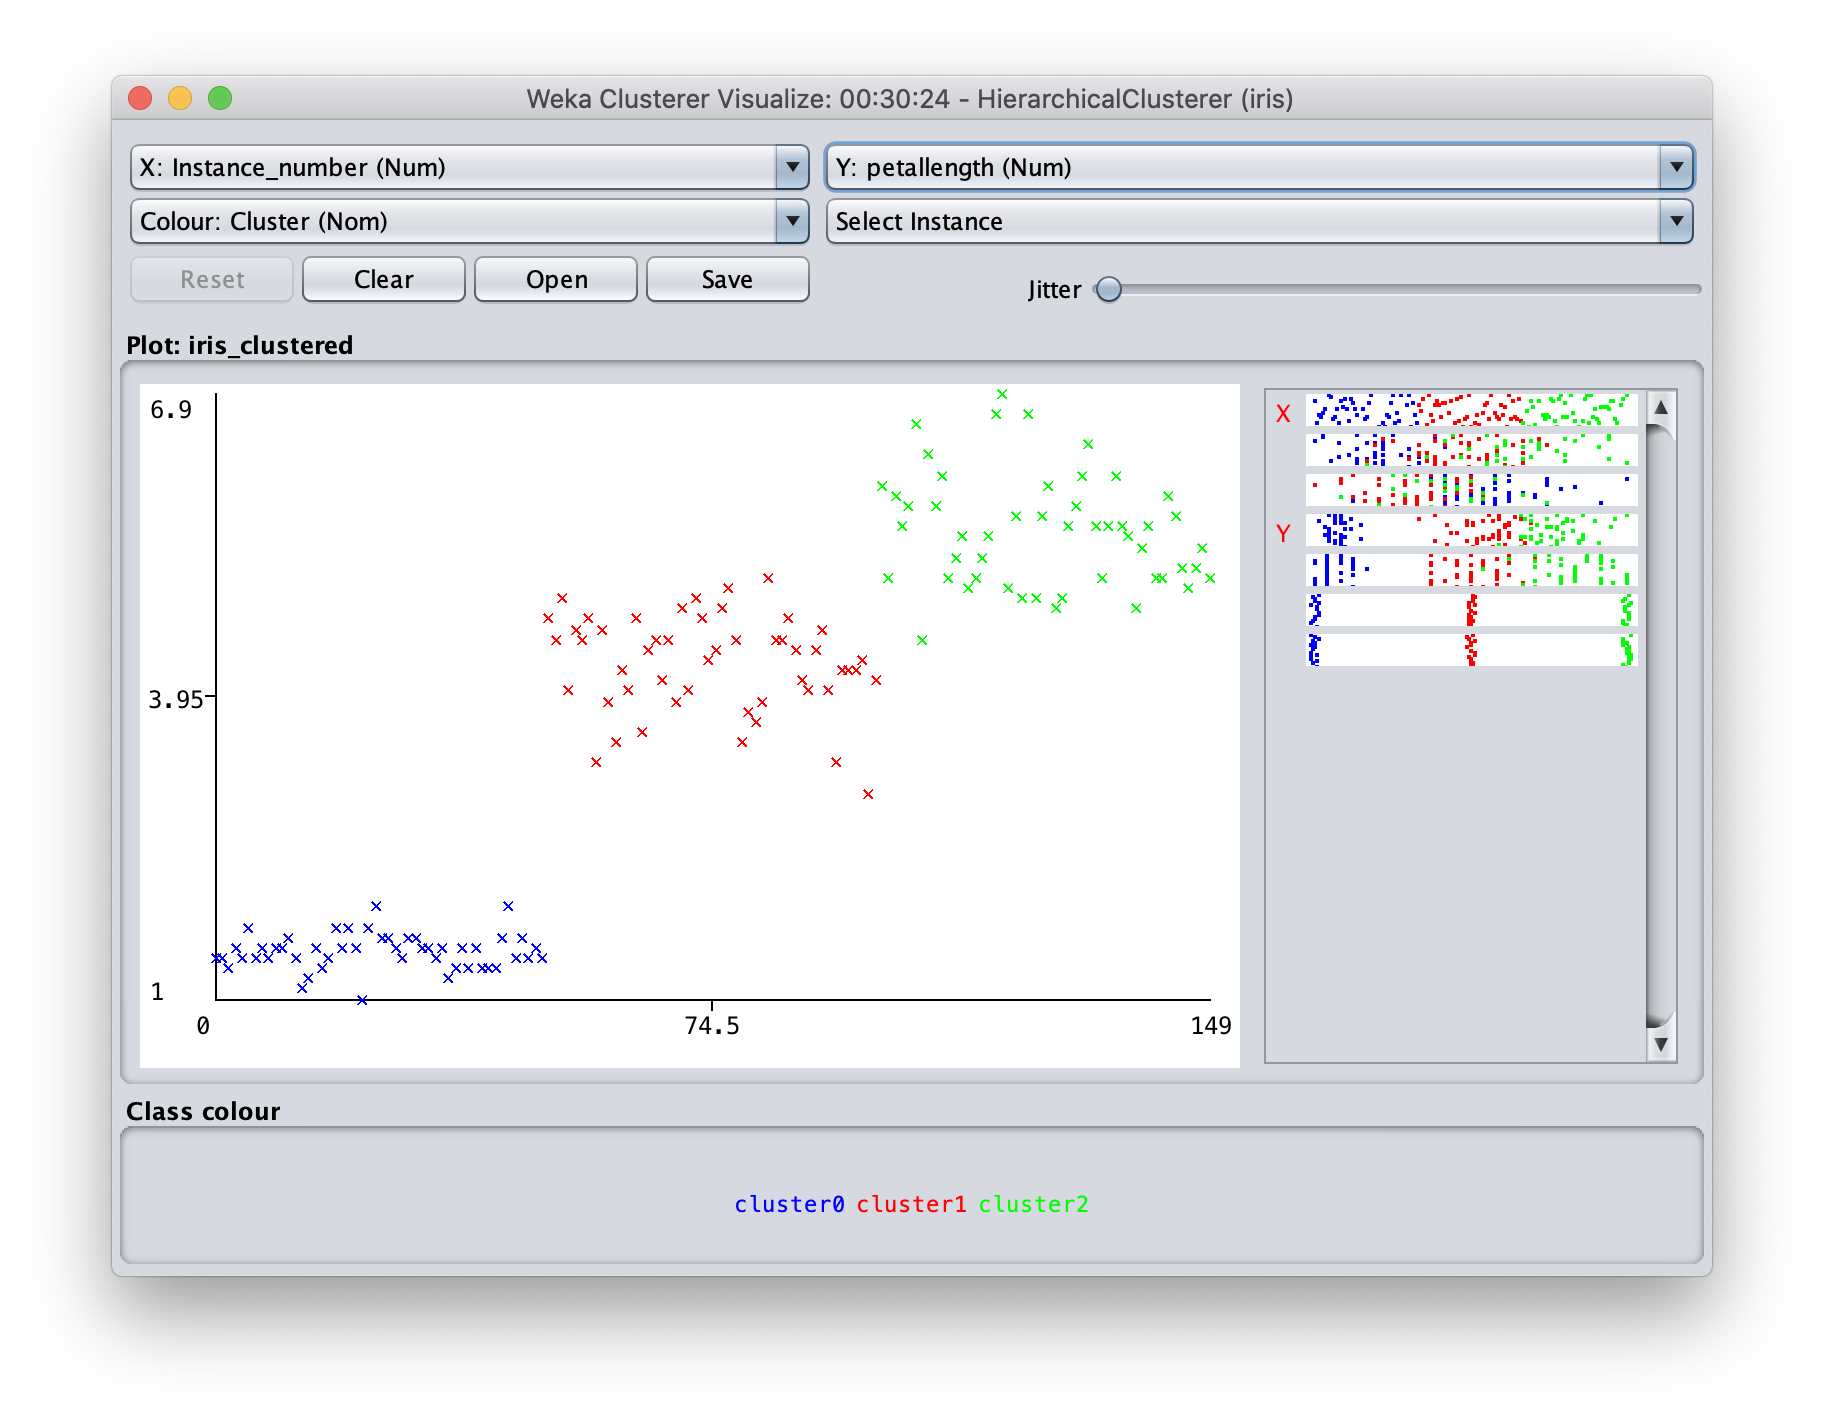
\includegraphics[width=0.6\textwidth]{hc_petallenght.png}
	\caption{X instance\_number con Y \textit{petallenght}.}
	\label{Captura_7}
\end{figure}

\begin{figure}[h]
	\centering
	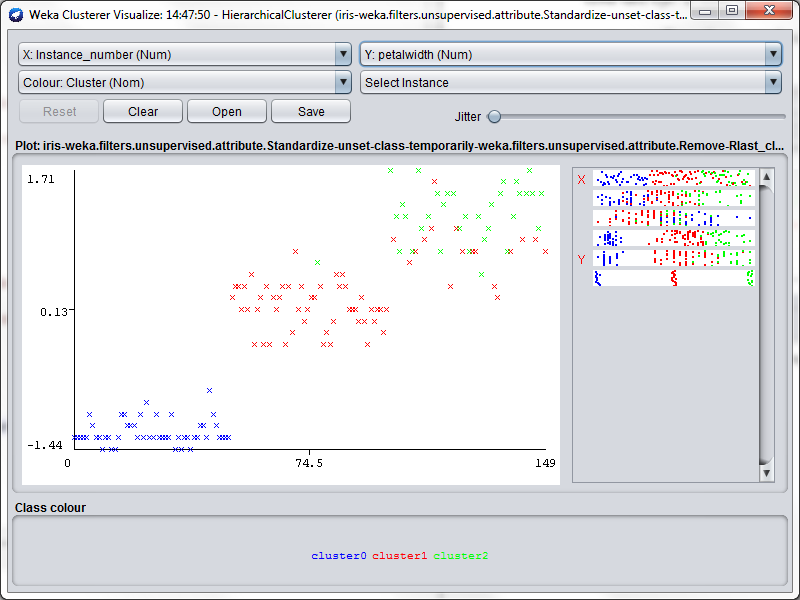
\includegraphics[width=0.6\textwidth]{hc_petalwidth.png}
	\caption{X instance\_number con Y \textit{petalwidth}.}
	\label{Captura_8}
\end{figure}

\begin{figure}[h]
	\centering
	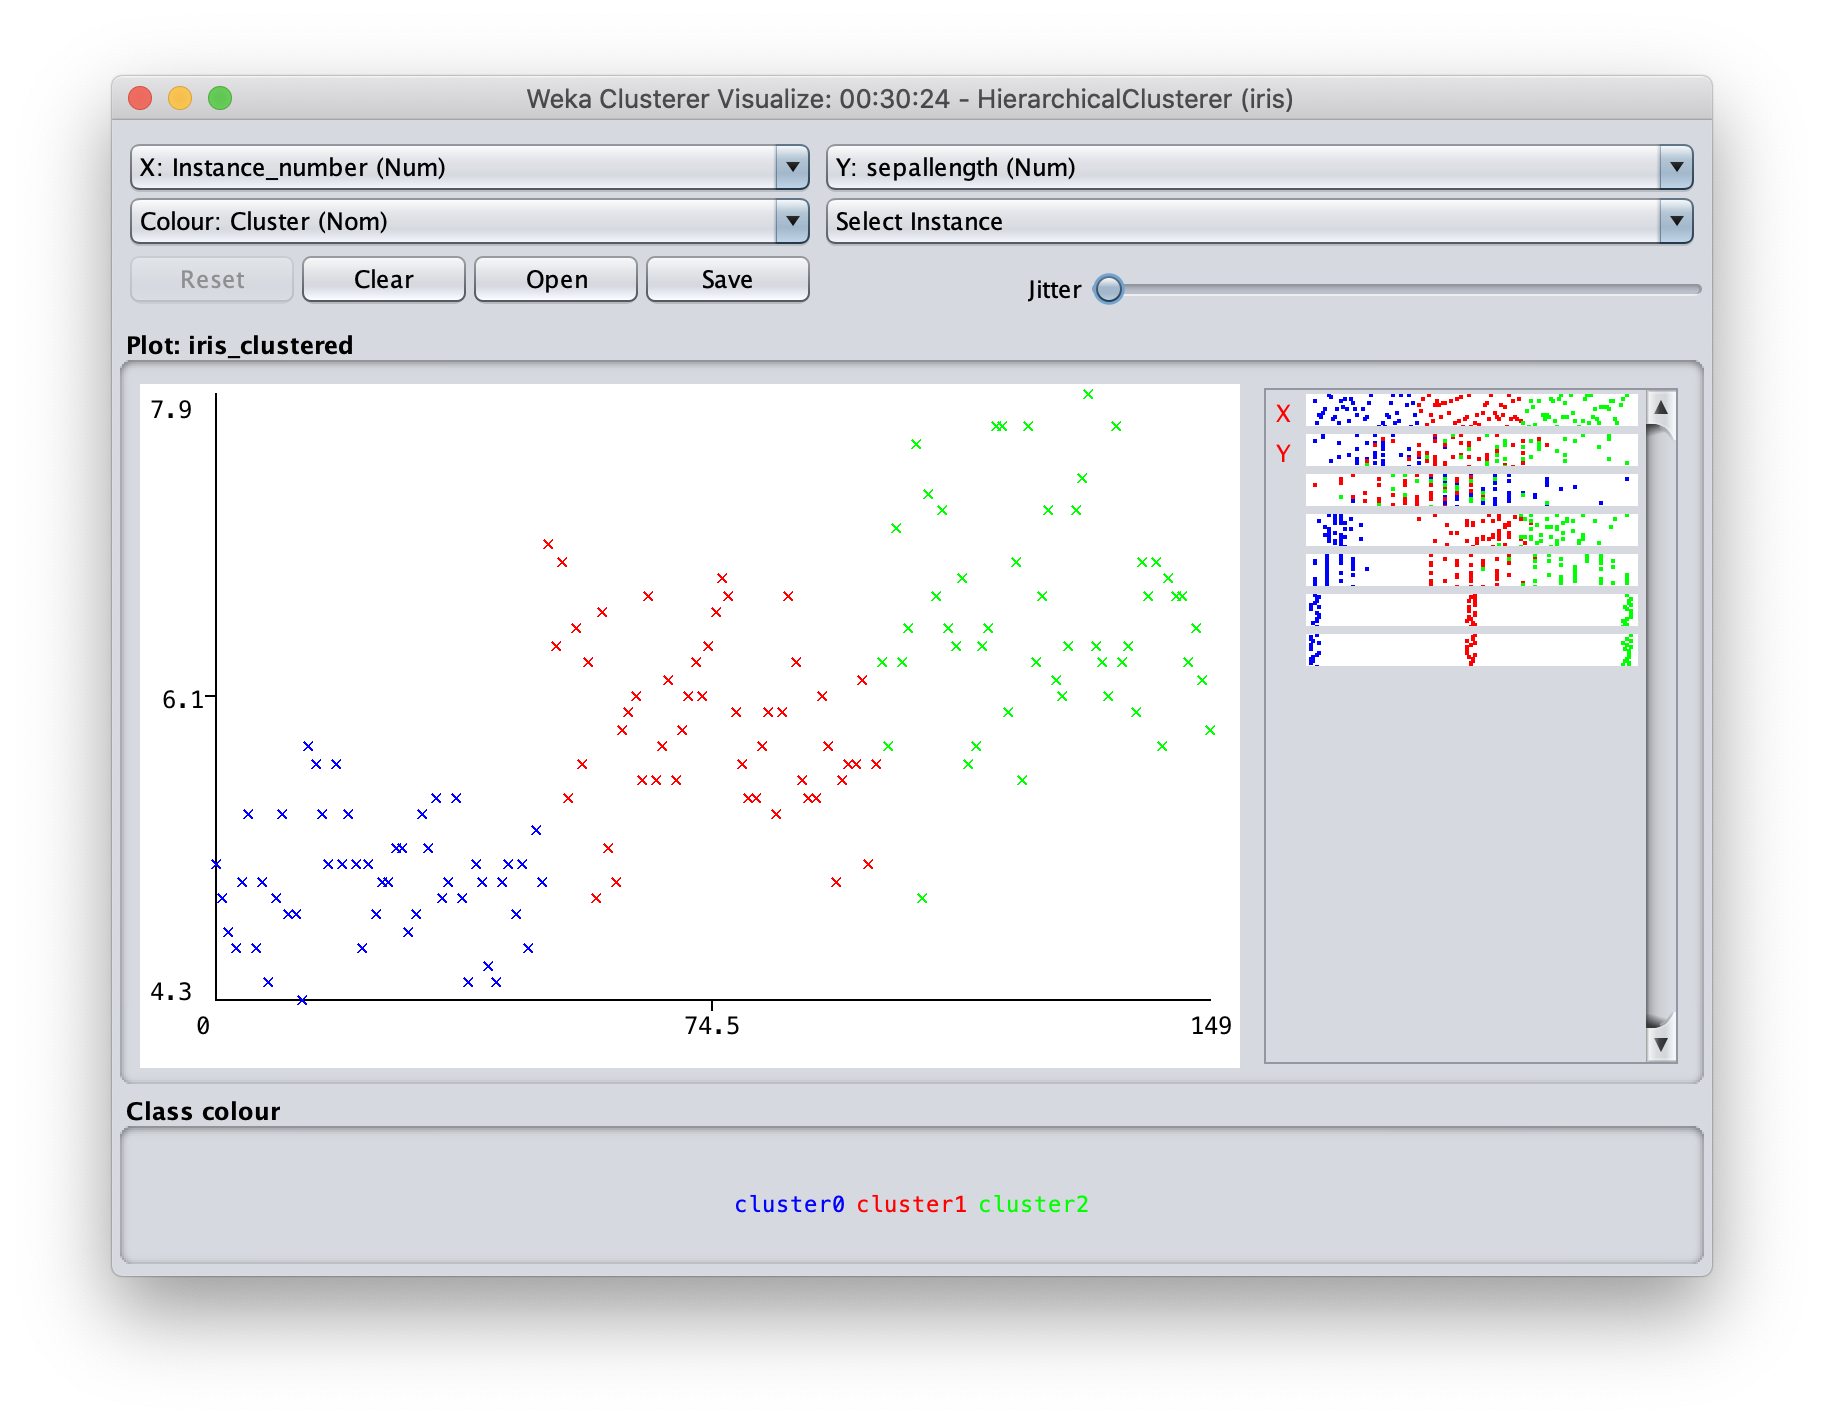
\includegraphics[width=0.6\textwidth]{hc_sepallebgth.png}
	\caption{X instance\_number con Y \textit{sepalleght}.}
	\label{Captura_9}
\end{figure}

\begin{figure}[h]
	\centering
	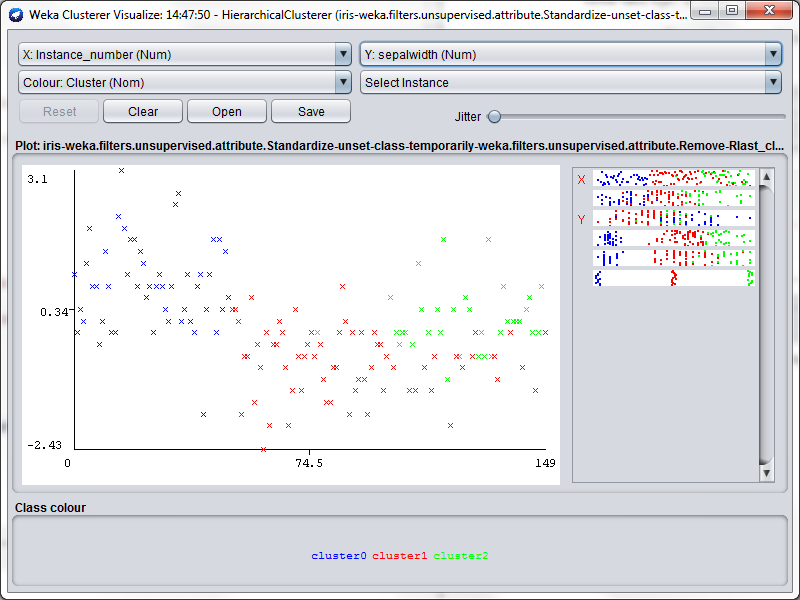
\includegraphics[width=0.6\textwidth]{hc_sepalwidth.png}
	\caption{X instance\_number con Y \textit{sepalwidth}.}
	\label{Captura_10}
\end{figure}

Las gráficas donde el eje Y es igual a las variables \textit{petallenght} i \textit{petalwidth} muestran grupos bien diferenciados y con las fronteras claras.

\end{questions}

\end{document}
